%% Encoding: ISO8859-1 %%

%% LaTeX-Beamer template for KIT design
%% by Erik Burger, Christian Hammer
%%
%% modified by Christian Henrich and Matthias Gabel for IKS/ITI
%%
%% version 1.3
%%
%% mostly compatible to KIT corporate design v1.2
%% http://www.uni-karlsruhe.de/download/uka/Gestaltungsrichtlinien_komplett.pdf

\documentclass[18pt]{beamer}
\usetheme{kit}

% if a custom picture is to be used on the title page, copy it into the 'logos'
% directory, in the line below, replace 'mypicture' with the 
% filename (without extension) and uncomment the line

 \renewcommand{\titleimage}{frontPic}

% (picture proportions: 63 : 20, *.eps format if you use latex+dvips+ps2pdf,
% *.jpg/*.png/*.pdf if you use pdflatex)

% if you want to see BibTeX keys in the references view instead of the symbol,
% uncomment the following line
% \usebibitemtemplate{\insertbiblabel}

% uncomment the following line if you want to hide the navigation symbols
%\beamertemplatenavigationsymbolsempty 

% the presentation starts here

\title[Short title]{Full title:\\ With all details}
\subtitle{??. ??. 201?}
\author{Firstname1 Lastname1, Firstname2 Lastname2}

\institute[ITI]{Fakult{\"a}t f{\"u}r Informatik, Institut f{\"u}r Theoretische Informatik} % Deutsch
%\institute[ITI]{Department of Informatics, Institute of Theoretical Informatics} % Englisch

\begin{document}

%\selectlanguage{english} % Deutsch
\selectlanguage{ngerman} % Englisch
%title page
\begin{frame}
	\titlepage
\end{frame}

%table of contents
\begin{frame}
	\frametitle{Outline/Gliederung}
	\tableofcontents
\end{frame}

%% Encoding: ISO8859-1 %%

\section{Grundlagen}

\frame{
\frametitle{Motivation}
    \begin{itemize}
        \item Energieeffiziente Schaltkreise f\"ur Nanoelektronik 
        \item Formales Modell basierend auf Petri Netzen
        \item Entwerfen von Schaltkreisen m\"oglichst einfach
    \end{itemize}
}

%---------------------------------------------------------------------

\frame{
\frametitle{Grundlagen}
    \begin{itemize}
        \item token basierte Schaltkreise (Bsp. Petri Netze)
        \item token pass Schaltkreise
        \item nicht polare token pass Brown'sche Schaltkreise
    \end{itemize}
}

%---------------------------------------------------------------------

\frame{
    \frametitle{Token basierte Schaltkreise}
    \begin{itemize}
        \item Signal als Token 
        \item asynchron (kein Takt)
    \end{itemize}

    \begin{figure}   
        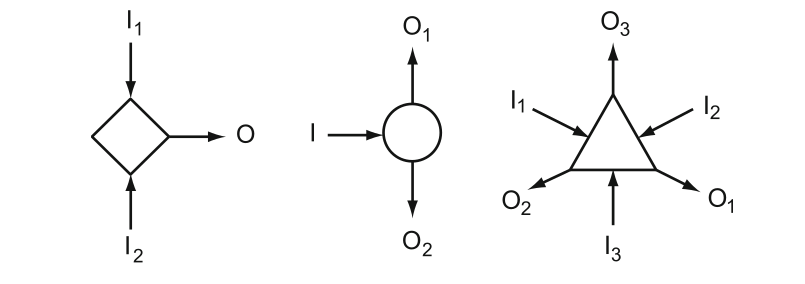
\includegraphics[width=7cm]{bilder/tokenBased.png}
        \caption{Merge, Fork und Tria}
    \end{figure}
}

%---------------------------------------------------------------------

\frame{
    \frametitle{Token pass Schaltkreise}
    \begin{columns}
        \begin{column}{.5\textwidth}
        \begin{itemize}
            \item Anzahl der Tokens immer gleich
            \item Tokens verlassen Kabel nicht
        \end{itemize}
        \end{column}
        \begin{column}{.5\textwidth} 
            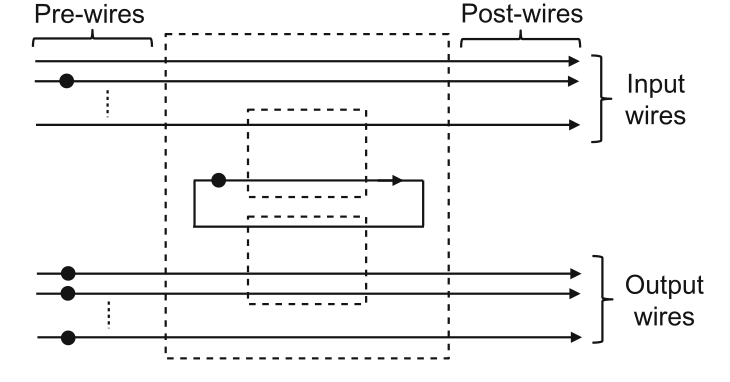
\includegraphics[width=6cm]{bilder/TokenPassScheme.png}
        \end{column}
    \end{columns}
}    

%---------------------------------------------------------------------

\frame{
    \frametitle{Von token basiert nach token pass}
    \begin{columns}
        \begin{column}{.5\textwidth}
            \begin{figure}
            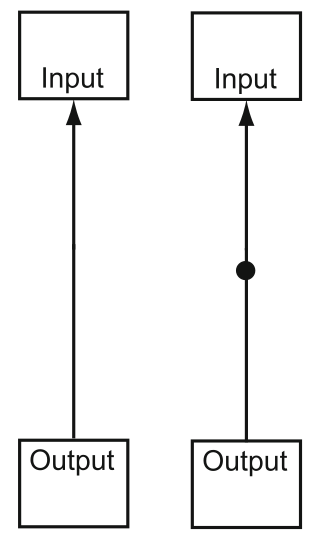
\includegraphics[width=3cm]{bilder/pass_based2.png}
            \caption{token basiert}
            \end{figure}
        \end{column}

        \begin{column}{.05\textwidth}
            \Huge
           $\Leftrightarrow$ 
        \end{column}

        \begin{column}{.5\textwidth} 
            \begin{figure}
            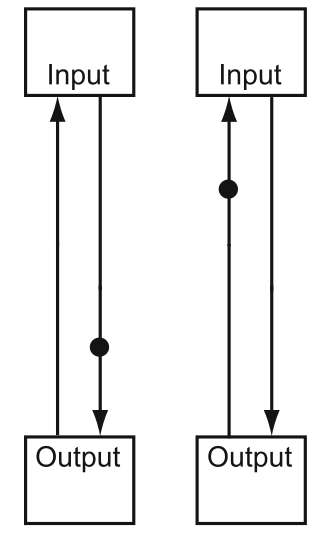
\includegraphics[width=3cm]{bilder/pass_based1.png}
            \caption{token pass}
            \end{figure}
        \end{column}
    \end{columns}
}

%---------------------------------------------------------------------

\frame{
    \frametitle{Brown'sche Schaltkreise}
        \begin{itemize}
            \item Tokens k\"onnen sich frei bewegen 
            \item Verz\"ogerungen beeinflussen nicht Korrektheit der 
                Berechnung
            \item Berechnungsschritte reversibel (Deadlocks)
        \end{itemize}
}

%---------------------------------------------------------------------

\frame{
    \frametitle{T-Element}
    \begin{columns}
        \begin{column}{.5\textwidth}
            \begin{figure}
            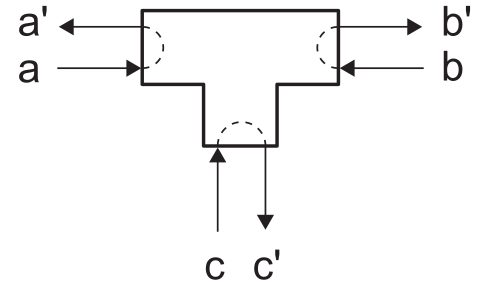
\includegraphics[width=5cm]{bilder/T-Element.png}
            \caption{T-Element}
            \end{figure}
        \end{column}
        \begin{column}{.5\textwidth} 
            \begin{figure}
            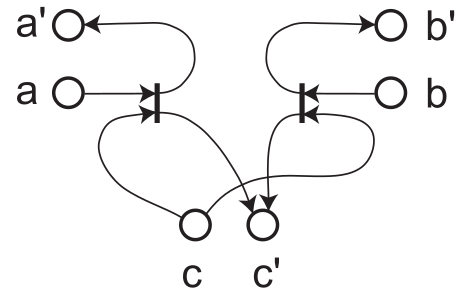
\includegraphics[width=5cm]{bilder/T_ElementPetri.png}
                \caption{als Petri-Netz}
            \end{figure}
        \end{column}
    \end{columns}
}

%---------------------------------------------------------------------

\frame{
    \frametitle{\"Aquivalenz von token basiert und token pass}
    \centering
    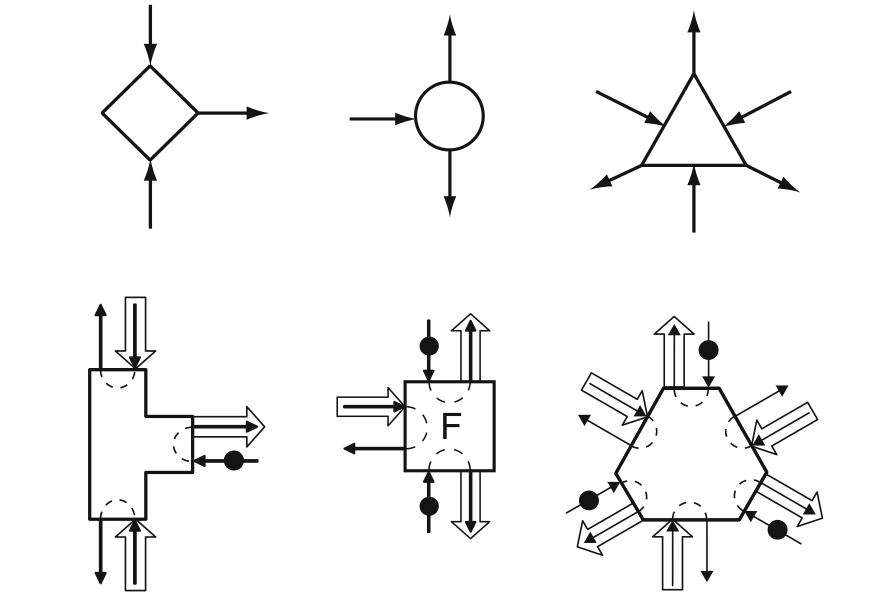
\includegraphics[width=8cm]{bilder/BasedToPass.png}

}

%---------------------------------------------------------------------

\frame{
    \frametitle{\"Aquivalenz von token basiert und token pass}
    \begin{figure}
        \begin{minipage}{0.45\textwidth}
            \centering
            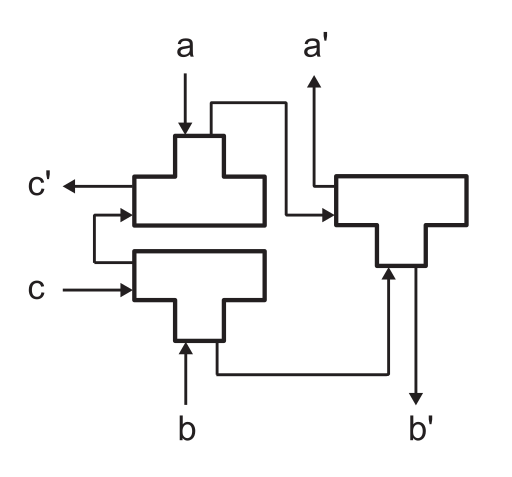
\includegraphics[width=5cm]{bilder/TP_Fork.png}
            \caption{Fork aus T-Elementen}
        \end{minipage}\hfill
        \begin{minipage}{0.45\textwidth}
            \centering
            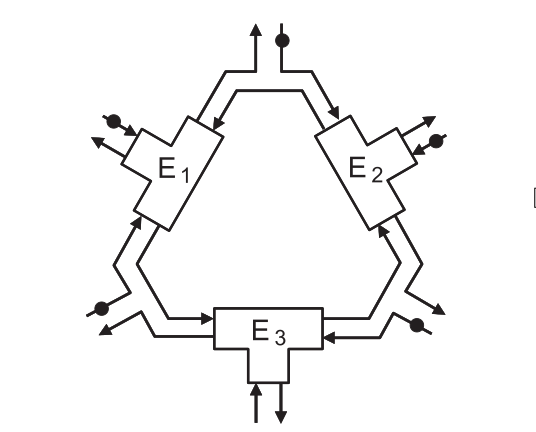
\includegraphics[width=5cm]{bilder/TP_Tria.png}
            \caption{Tria aus T-Elementen}
        \end{minipage}\hfill
    \end{figure}
}

%--------------------------------------------------------------------

\frame{
\frametitle{\"Aquivalenz von token basiert und token pass}
T-Element ist Schaltkreisprimitiv f\"ur brown'sche token pass 
Schaltkreise 
}

%--------------------------------------------------------------------

\frame{
    \frametitle{Nicht polare token pass Schaltkreise}
    \begin{columns}
        \begin{column}{.5\textwidth}
            \begin{itemize}
                \item Tokens haben keinen Bias mehr 
                \item Terminator Kabel 
                \item Bias auf Ein- und Ausgabekabeln sinnvoll
            \end{itemize}
        \end{column}

        \begin{column}{.5\textwidth} 
            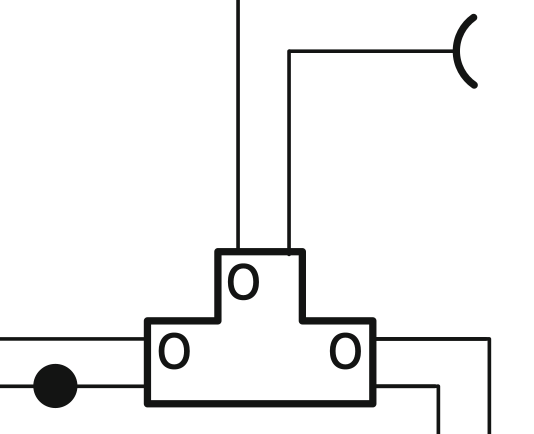
\includegraphics[width=5cm]{bilder/NonPolarTerminator.png}
        \end{column}
    \end{columns}

}

%--------------------------------------------------------------------

\frame{
    \frametitle{Nicht polar token pass Schaltkreise}
T-Element ist Schaltkreisprimitiv f\"ur brown'sche token pass 
Schaltkreise 
}


%--------------------------------------------------------------------
%---------------------------------------------------------------------


\section{1-Bit Speicher}

\frame{
    \frametitle{Nicht polarer 1-Bit Speicher}
    \centering
    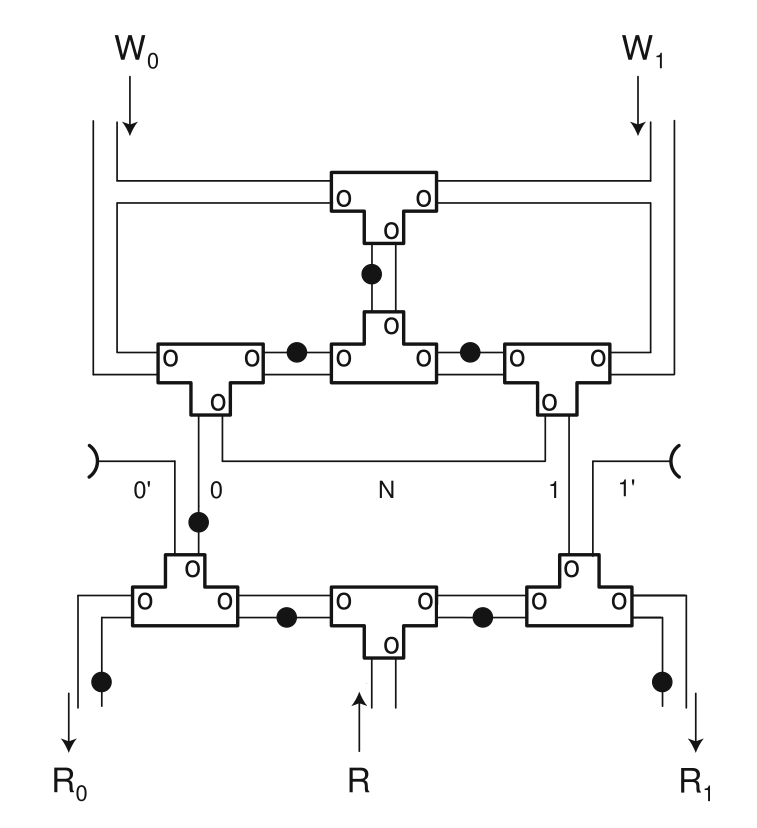
\includegraphics[width=6.5cm]{bilder/NonPolarMemory.png}
}

%---------------------------------------------------------------------

\frame{
    \frametitle{Lesen einer 0}
    \begin{figure}[ht]
        \begin{overlayarea}{7cm}{5cm}
            \includegraphics[width=6.5cm]<1>{bilder/1BitSpeicher/Read_1.png}
            \includegraphics[width=6.5cm]<2>{bilder/1BitSpeicher/Read_2.png}
            \includegraphics[width=6.5cm]<3>{bilder/1BitSpeicher/Read_1.png}
            \includegraphics[width=6.5cm]<4>{bilder/1BitSpeicher/Read_3.png}
            \includegraphics[width=6.5cm]<5>{bilder/1BitSpeicher/Read_4.png}
            \includegraphics[width=6.5cm]<6>{bilder/1BitSpeicher/Read_5.png}
        \end{overlayarea}
    \end{figure}
}

%---------------------------------------------------------------------

\frame{
    \frametitle{Schreiben einer 1}
    \begin{figure}[ht]
        \begin{overlayarea}{7cm}{7cm}
            \includegraphics[width=6cm]<1>{bilder/1BitSpeicher/Write_1.png}
            \includegraphics[width=6cm]<2>{bilder/1BitSpeicher/Write_2.png}
            \includegraphics[width=6cm]<3>{bilder/1BitSpeicher/Write_3.png}
            \includegraphics[width=6cm]<4>{bilder/1BitSpeicher/Write_2.png}
            \includegraphics[width=6cm]<5>{bilder/1BitSpeicher/Write_4.png}
            \includegraphics[width=6cm]<6>{bilder/1BitSpeicher/Write_5.png}
            \includegraphics[width=6cm]<7>{bilder/1BitSpeicher/Write_6.png}
        \end{overlayarea}
    \end{figure}
}

%---------------------------------------------------------------------
%---------------------------------------------------------------------

\section{UND-Gatter} 

\frame{
    \frametitle{UND-Gatter}
    \begin{itemize}
        \item Repr\"asentation von 1 als Token und 0 als Abwesenheit
        \item Repr\"asentation von 1 und 0 als Token 
        \item Ausnutzen des Backtrackings aus Deadlocks
    \end{itemize}
}

%---------------------------------------------------------------------

\frame{
    \frametitle{0 durch kein Token repr\"asentiert}
    \centering
    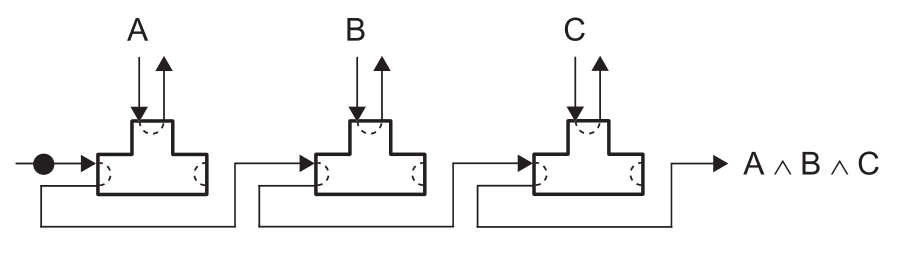
\includegraphics[width=9cm]{bilder/UND_simple.png}
}

%---------------------------------------------------------------------

\frame{
    \frametitle{0 und 1 durch Token repr\"asentiert}
    \centering
    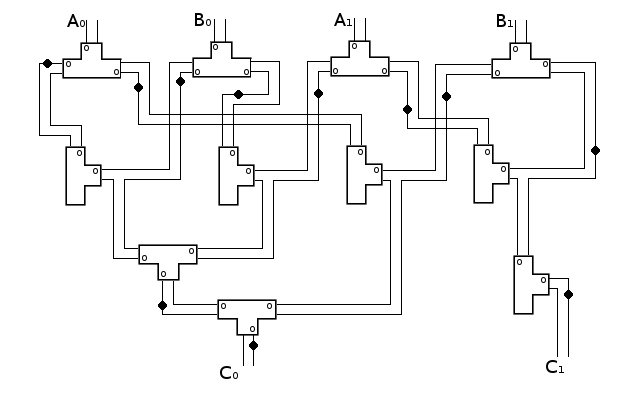
\includegraphics[width=10cm]{bilder/UndGatterOhneRand.png}
}

%---------------------------------------------------------------------

\frame{
    \frametitle{0 und 1 durch Token repr\"asentiert}
    \centering
    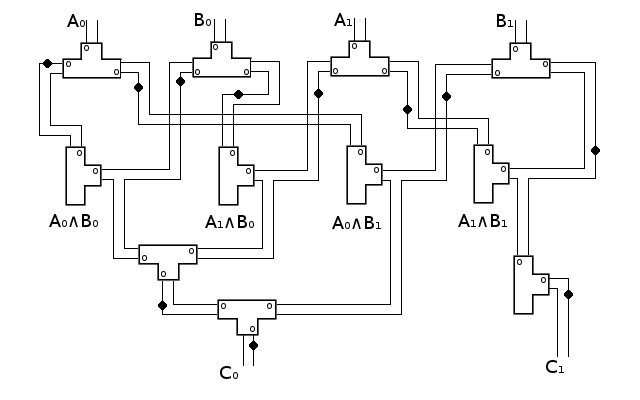
\includegraphics[width=10cm]{bilder/UndGatterOhneRandBeschriftung.png}
}


%---------------------------------------------------------------------
%---------------------------------------------------------------------

\section{Ausblick}

\frame{
    \frametitle{Geschwindigkeit der Berechnung}
    \begin{itemize}
            %TODO
        \item Ausnutzen von Bias bei Ein- und Ausgabekabeln
        \item zus\"atzlich Sperren (Kabel nur in eine Richtung)
        \item wie effizient ist backtracking aus Deadlocks?
    \end{itemize}
}

%---------------------------------------------------------------------

\frame{
    \frametitle{Konkrete Implementierung}
    \begin{itemize}
        \item Ans\"atze mit einzelne Elektronen
            \begin{itemize}
                \item Problem: Token wirken aufeinander 
            \end{itemize}
    \end{itemize}
}

%---------------------------------------------------------------------

\frame{
    \frametitle{Korrektheit}
    \begin{itemize}
        \item wann ist Berechnung vorbei?
        \item kann startkonfiguration immer gew\"ahrleistet werden?
    \end{itemize}
}


%---------------------------------------------------------------------
%---------------------------------------------------------------------


\section{Zusammenfassung} 

\frame{
    \frametitle{Zusammenfassung}
    \begin{itemize}
        \item Brown'sche Schaltkreise f\"ur Elektronik im Nanometer Bereich
        \item Nicht polare Brown'sche Schaltkreise erm\"oglichen
              einfacheres Desgin
        \item Korrektheit, Geschwindigkeit etc noch ungekl\"art
    \end{itemize}
}



\begin{frame}
	\frametitle{References}
	\bibliography{example}
%	\bibliographystyle{plain} %does not render "url" fields...
	\bibliographystyle{IEEEtran}  %does render "url" fields, requires "_"s and "#"s to be escaped, e.g. "\_".
\end{frame}

\end{document}

